\section{Experiments}~\label{experiment}
Our experiments evaluate the proposed system from two complementary perspectives, system-level performance and human-user interaction. The system evaluation uses an oracle user to isolate the behavior of the planning and query framework under controlled feedback. We measure task success, the number of queries, query rate, and planning length to examine the trade-off between task performance and interaction cost. The user study examines how the resulting query interaction affects participant performance, workload, and situation awareness in practical task settings.


\begin{figure}[t!]
    %\captionsetup{skip=0pt} % \hspace{0.3cm}
    \begin{center}
  
    \begin{subfigure}[b]{0.47\textwidth}
        \captionsetup{skip=0pt}
	    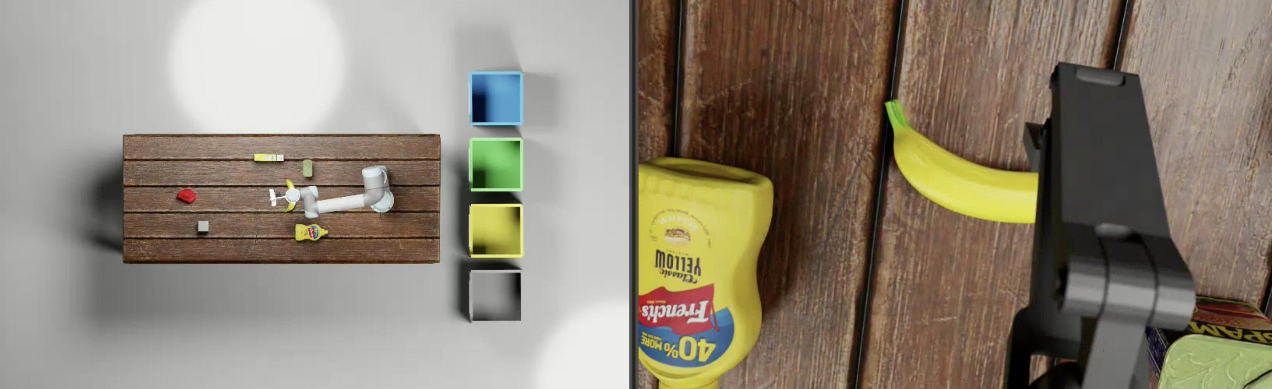
\includegraphics[width=\textwidth]{figures/intro_and_method/fig_exp_setup1.pdf}
        \caption{Waste sorting domain overview. }
        \label{fig:dom1}
    \end{subfigure}
    \quad
    \begin{subfigure}[b]{0.47\textwidth}
        \captionsetup{skip=0pt}
	    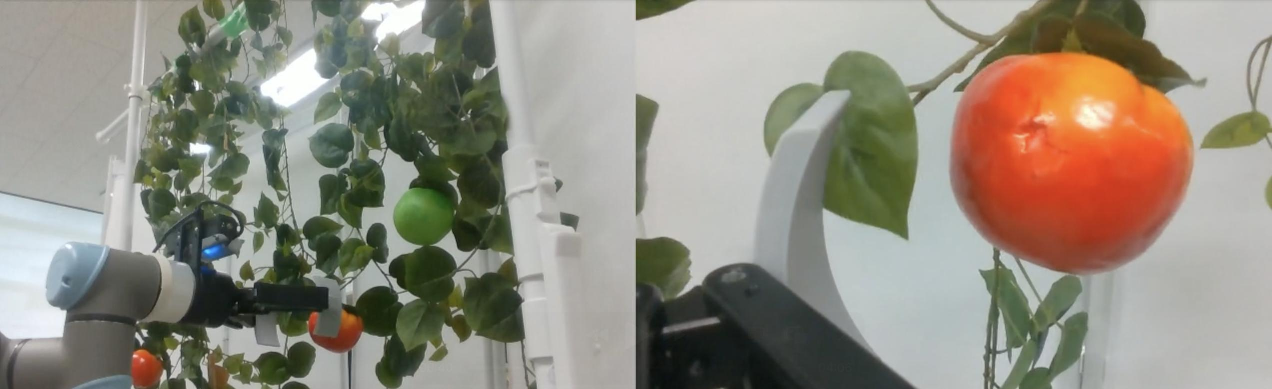
\includegraphics[width=\textwidth]{figures/intro_and_method/fig_exp_setup2.pdf}
        \caption{Tomato harvesting domain overview}
        \label{fig:dom2}
    \end{subfigure}
    \caption{The illustration of the environments. (a) A UR5 robot sorts four types of waste into designated bins in Isaac Sim. (b) A mobile manipulator harvests ripe tomatoes and discards rotten ones in a real-world setting.}
  \label{fig:env_setting}
  
  \end{center}
\end{figure}


\subsection{Experimental Setup}~\label{exp:setup}
We evaluate the framework in two task domains, waste sorting and tomato harvesting, using controlled system-level environments for repeated trials. The waste sorting domain is implemented in NVIDIA Isaac Sim with a tabletop scene and a fixed UR5 robotic arm for pick-and-place tasks. The tomato harvesting domain follows the task structure and sensing setup of our real robot platform, which consists of a Summit mobile base, a UR5e arm, an RGB-D camera, and a LiDAR sensor. The repeated system-level evaluations are conducted in a controlled environment to support randomized trials and fair comparisons across conditions. Both domains use YOLOv12 for object detection~\cite{tian2025yolov12}.


\subsubsection{Waste sorting domain}~\label{exp:setup_waste}
As shown in Fig.~\ref{fig:dom1}, a fixed UR5 robot is positioned between the objects and the recycling bins and performs three actions: \texttt{detect}, \texttt{pick}, and \texttt{place}. We assume that all objects are reachable by the manipulator.

Each object belongs to one of four categories: \texttt{general}, \texttt{paper}, \texttt{can}, and \texttt{plastic}. The object categories are not known a priori and must be inferred through perception. Since objects may be partially occluded by others, a single observation may not reveal all categories, requiring repeated detection during execution. The \texttt{detect} action can observe multiple objects simultaneously, after which the robot places each object into the corresponding recycling bin.

The initial arrangement of objects is randomized in every episode. A task is considered successful when all objects are correctly sorted within the maximum step limit. A reward of $+5$ is assigned when a waste object is placed into the recycling bin corresponding to its category, and an additional reward of $+10$ is given when all objects are correctly sorted. All other actions receive zero reward.



\subsubsection{Tomato harvesting domain}~\label{exp:setup_tomato}
We consider a tomato harvesting scenario in which four tomatoes are attached to two stems, denoted as \texttt{stem\_1} and \texttt{stem\_2}, as shown in Fig.~\ref{fig:dom2}. The robot navigates between three locations: \texttt{dock\_station}, \texttt{stem\_1}, and \texttt{stem\_2}, and performs \texttt{detect}, \texttt{pick}, \texttt{scan}, \texttt{place}, and \texttt{discard} actions.

Each tomato can be in one of three states: \texttt{ripe}, \texttt{unripe}, or \texttt{rotten}. The tomato states are initially unknown and must be estimated through perception. During detection, ripe and rotten tomatoes are visually ambiguous and cannot always be reliably distinguished. To resolve this ambiguity, the robot performs a \texttt{scan} action after picking a tomato to verify its condition before harvesting or discarding it. Unripe tomatoes are left untouched.

The tomato locations are randomized across stems in every episode. A task is considered successful when all ripe tomatoes are harvested and all rotten tomatoes are discarded within the maximum step limit. A reward of $+5$ is assigned when a ripe tomato is correctly harvested or a rotten tomato is correctly discarded after scanning. An additional reward of $+10$ is given when all task-relevant tomatoes are processed correctly. All other actions receive zero reward.



\subsubsection{Implementation Details}~\label{exp:details}
In all experiments, the planner used a discount factor $\gamma=0.95$, UCB exploration constant $c=1.0$, maximum simulation depth $depth_{\max}=20$, and $\Timeout=100$ Monte Carlo simulations per planning step. Each standard episode was limited to $50$ steps. Each reported threshold or policy result aggregates five scenario configurations with $40$ randomized episodes per scenario, yielding $200$ episodes per domain-condition cell. Randomized episodes are generated from logged pseudorandom seeds. Detailed implementation settings are provided in Appendix~\ref{appx:settings}.
